\section{Experiment}
\label{sec:experiment}

\subsection{Data Set}

We evaluated our system on two data sets: the HKUST Mandarin Telephone Speech corpus and the PAEC financial phone call data set collected by Ping An Technology (Shenzhen) Co.,Ltd China.

\begin{itemize}

\item HKUST corpus: HKUST corpus \cite{Liu2006HKUST} is a large scale Mandarin speech corpus which comprises around 200 hours of telephone recordings, with over 2100 Mandarin speakers and including 1206 ten-minute phone call conversations, recorded at an 8k sampling rate, where the two callers do not know each other in advance. Most of the phone calls are recorded from relatively quiet environments. All channel A wav data are used to train UBM. We split out all channel B wav data to five 30-second sub-recordings and abandon the rest.

\item PAEC corpus: The PAEC data set is a building financial phone call conversations between customer and service staff in the field of banking, insurance and other financial business. Phone calls are recorded from variational environment in 8k sampling rate. For customers, many are using mobile phones or land-line phones, while for Ping An service staffs they use lapel microphones. The data set we used to train and test our system consists of 900 speakers with 40 hours multi-calls for each in training set and 5 hours uni-call for each in test set. Meanwhile, to test the accuracy of customer/service identification module, 900 customer/service dialogues (text) are transcribed from these audio by ASR model and 32,445 segments (short text) are extracted from these dialogues. Each segment is manually assigned ``customer" or ``service" label.

\end{itemize}

All experiments are performed on a Intel Core 8 processor Linux machine, 64 GB memory and all these experiments are run 10 times and then calculate the average score.

\subsection{Experiment Results}

Our first experiment shows the performance of various kinds of DNN-UBM versus GMM-UBM baseline speaker verification system. The Equal Error Rate (EER) \cite{Dehak2010Cosine} index is applied to evaluate speaker verification system.

The experiment setup for various text-independent speaker verification pipeline can be described as follow.

\begin{itemize}
\item GMM-UBM baseline: the feature front-end is 40-dimension MFCC vector with delta and delta-delta. VAD method is applied after feature extraction step. We set the UBM 2048 components and for i-vector dimension is 600-dimension. At the end, a cosine similarity scoring back-end is used to evaluate the system performance.

\item  DNN-UBM: we compared various deep neural networks within DNN-UBM applied in text-independent speaker verification system. The DNN feature is generated as 40-dimension FilterBank vector, VAD method is applied as the same. For DNN-UBM components, we set all neural network model output (number of senone states)to 3000 (this is depended on the last GMM-HMM decision tree clusters, various from different training set, so it might be slightly different to 3000, i.e. for HKUST corpus the number is 2798, for Ping An corpus the number is 2825, there is no harm with a closed difference, we just want to choose closed to the 2048 of GMM-UBM baseline components). The rest of i-vector and scoring back-end stay the same as above.

1) MN-UBM: the MN abbreviation indicates the maxout network, with introduced p-norm generalized maxout units as described in \cite{Zhang2014Improving}. The test MN has 5 hidden layers, and the p-norm input dimension is 3000, p-norm output dimension is 300.

2) TDNN-UBM: the time-delay neural network used to test consists of 7 layers, for different layers, the splice indexes are represented as ``-2,-1,0,1,2 -1,2 -3,3 -7,2 -3,3 0 0". The hidden layers have an input dimension of 300 and an output dimension 3000.

3) HLSTM-UBM: the highway lstm recurrent neural network has the same structure as LC-HBLSTM described in the ASR module section. It has 5 layers, with 1024 memory cells together with a 512-node projection layer at each layer��s output. The output targets are 3k dimensional context-dependent tied triphone states.

4) BLSTM-UBM: the BLSTM components are similar to HLSTM-UBM, it has 5 hidden layers, each layer consists of 1024 memory cells (512 for forward and 512 for backward) with a 512-node projection layer.

\end{itemize}


\begin{table}[!hbp]
\caption{EER(\%), response time between GMM-UBM and DNN-UBM}
\centering
\begin{tabular}{|c|c|c|c|}
\hline
& HKUST data set & Ping An data set & response time\\
\hline
GMM-UBM & 0.1116\% & 5.63\% & 408ms \\
\hline
MN-UBM & 0.1115\% & 5.27\% & 637ms \\
\hline
TDNN-UBM & 0.1107\% & 4.83\% & 593ms \\
\hline
\textbf{HLSTM-UBM} & 0.1109\% & \textbf{4.69\%}& \textbf{585ms} \\
\hline
BLSTM-UBM & 0.1100\% & 4.56\% & 1359ms \\
\hline
\end{tabular}
\label{tab:accuracyGMMHLSTM}
\end{table}

As one should know, the HKUST corpus is well designed for ASR task, but may not be the best corpus to verify SV due to the lack of speaker channel difference, that is, in HKUST we do not have multi-calls per speaker. We guess that is why in both all test case the EERs stay quite closed (0.1100\% - 0.1115\%).

Table \ref{tab:accuracyGMMHLSTM} shows the EER and response time comparison from GMM-UBM baseline and various DNN-UBM i-vector based SV system. From the results we find that the DNN-UBM has an average of 15\% relative improvement from GMM-UBM baseline. BLSTM-UBM achieves the bast equal error rate of 4.56\% in Ping An test set, while TDNN-UBM (4.83\%) and HLSTM-UBM (4.69\%) performs closed.

However, since the response time is very important in Ping An Telephone Customer Service (The response time is the time for test, rather than training time.) Our second experiment focuses on the response time of GMM-UBM and various DNN-UBM. From table \ref{tab:accuracyGMMHLSTM}, we find that when apply the same test data, e.g. one 30s clean single track audio, BLSTM-UBM (1359ms) performs more than 3 times compared to the other type of SV systems, while HLSTM-UBM's response time is just a little slower than GMM-UBM system (408ms for GMM-UBM and 637ms for HLSTM-UBM.) Since both response time is less than 1s, HLSTM-UBM with much higher accuracy can be used in the real telephone service system.

Experiment 3 analyze the performance of short text classification. $F_{1}$ \cite{Li2008Learning}, which is the harmonic average of the precision $p$ and recall $r$, is used to evaluate this binary (service/customer) classification.

We conducted experiments on PAEC data set, which has manually been labeled customer/service. We evaluate three schemes to set the weight for the query (short-text in test data): Boolean, TF, TF.IDF \cite{Salton1988Term}. Meanwhile, various $k$ value has also been tested in this experiment. The classification accuracy (F1 score) are reported in Figure  \ref{fig:F1score}. From the results, we have the following observation. First, all the methods receive the very high accuracy (more than 0.93.) Since the dialog between various customer and service are much similar in TCS, ``word matching" technique will receive the high accuracy. Second, as we know, $k$ value is an important character for KNN algorithm. Using $k = 1$, our approach gets a poor result (0.93) since the very less votes has been considered in the experiments. However, the accuracy for $k$ in (3, 5, 7) are much similar, since three voting is enough for KNN classification algorithm. Third, TF-KNN and Boolean-KNN receives much similar accuracy, since the same terms in each query only appears one to two times (Remember TF is the term frequency.) Both TF-KNN and Boolean-KNN get the higher accuracy than TF.IDF-KNN. IDF is low when this term (a normal term) appears to the various short text. However, a normal term does not mean this word is not important for the classification. For example, ``apply" appears for the various short texts, but it is easy to identify the customers by this term. In sum, with the high accuracy, KNN-TF ($k$=3) is used in the following experiments.

\begin{figure}
\centering
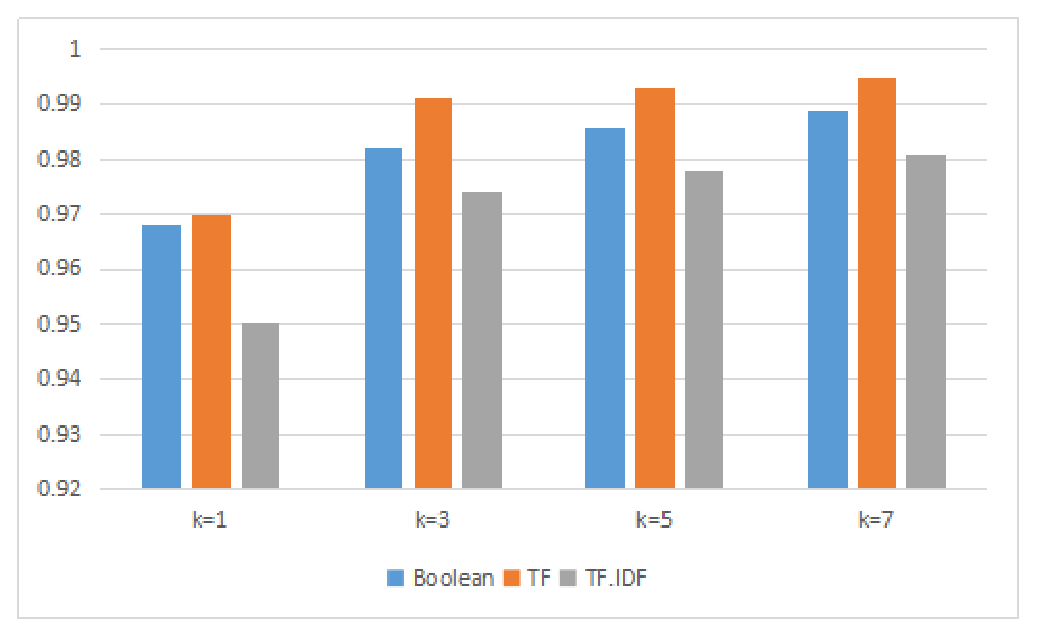
\includegraphics[width=3.5in]{figures/f1Score.eps}
\caption{F1 Score for Short Text Classification}
\label{fig:F1score}
\end{figure}

Experiment 4 compares different methods for co-channel case. In this experiment, three methods has been compared.

\begin{itemize}
\item Baseline 1: mixed audio, which including customer and client service in one single channel.

\item Baseline 2: the first customer utterance (average 4.4s in PAEC) extracted from the mixed audio in Baseline 1. In PAEC corpus, the first utterance is always belonged to the client service, so that we applied sequential gaussian mixture model based voice activity detection method and cut the second utterance as the customer��s first utterance segment.

\item Our Approach: the concatenated customer speech from our SV framework. The mixed\_* represents how long our input mixed audio is. For example, mixed\_60 means that the mixed audio is about 60s.


\end{itemize}

The experimental results are shown in Figure \ref{fig:ERRForThreeMethods}. We have the following observation:  (i) It is clear that baseline 1 obtains the lowest accuracy (err is 64.2\%) since for the mixed data the SV system cannot judge the data stand for which speaker is. (ii) Baseline 2 shows the short utterance effects on speaker recognition. As the utterances get shorter (average 4.4s), results deteriorate (err is equal to 13.2\%.) (iii) Our approach (mixed\_60s\footnote{The average length of concatenated customer speech segments is around 39.6s in PAEC data set.}) performs much better than that the other two baseline, since we concatenate more clean target speaker data, making the audio length increased, the result improve dramatically, which closed to the original cleaned single track performance (compare to table \ref{tab:accuracyGMMHLSTM}.)

Since in Ping An's financial business, different departments have various need for balancing accuracy with response time, We also list the effect of various length of the input mixed co-channel audio in Figure \ref{fig:ERRForThreeMethods}. From mix\_10 to mix\_30, the err ratio decreases dramatically (from 11.8\% to 5.4\%.) However, from mix\_30 to mix\_60, the err ratio decreases slowly (from 5.4\% to 4.5\%). Therefore, 30s mixed audio is used in our real telephone customer service.

\begin{figure}
\centering
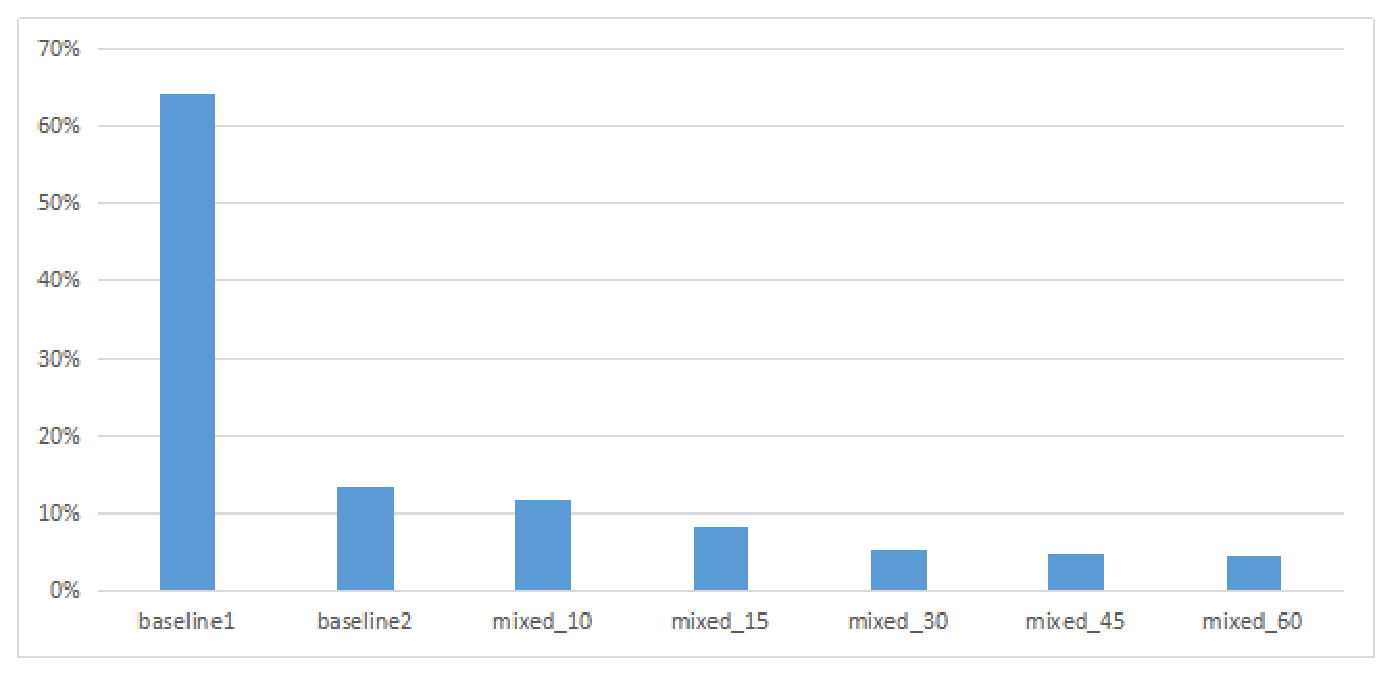
\includegraphics[width=3.5in]{figures/ERRForThreeMethods.eps}
\caption{ERR(\%) for Three Approaches}
\label{fig:ERRForThreeMethods}
\end{figure}
